\documentclass[11pt]{article}
\usepackage[margin=1in]{geometry}
\usepackage{amsmath,amssymb,amsthm,mathtools}
\usepackage{booktabs}
\usepackage{array}
\usepackage{xcolor}
\usepackage{enumitem}
\usepackage{tikz}
\usetikzlibrary{arrows.meta,patterns,decorations.pathreplacing}
\usepackage[protrusion=true,expansion=false]{microtype}
\usepackage[hidelinks]{hyperref}

\theoremstyle{plain}
\newtheorem{theorem}{Theorem}[section]
\newtheorem{proposition}[theorem]{Proposition}
\newtheorem{lemma}[theorem]{Lemma}
\newtheorem{corollary}[theorem]{Corollary}
\theoremstyle{definition}
\newtheorem{definition}[theorem]{Definition}
\theoremstyle{remark}
\newtheorem{remark}[theorem]{Remark}

\definecolor{forcedc}{RGB}{15,110,86}
\definecolor{declaredc}{RGB}{24,95,165}
\definecolor{openc}{RGB}{163,45,45}
\definecolor{growc}{RGB}{31,138,107}
\definecolor{capc}{RGB}{62,134,200}
\newcommand{\forced}{\textcolor{forcedc}{\textsc{[forced]}}}
\newcommand{\computed}{\textcolor{forcedc}{\textsc{[computed]}}}
\newcommand{\declared}{\textcolor{declaredc}{\textsc{[declared]}}}
\newcommand{\openq}{\textcolor{openc}{\textsc{[open]}}}

\newcommand{\R}{\mathbb{R}}
\newcommand{\Q}{\mathbb{Q}}
\newcommand{\Z}{\mathbb{Z}}
\newcommand{\Cx}{\mathbb{C}}
\newcommand{\D}{\mathbb{D}}
\newcommand{\Mah}{\mathrm{M}}
\newcommand{\spec}{\operatorname{spec}}
\newcommand{\ad}{\operatorname{ad}}
\newcommand{\Scal}{\mathcal{S}}
\newcommand{\abs}[1]{\left\lvert #1 \right\rvert}
\newcommand{\trace}{\mathsf{tr}_{\!\downarrow}}

\title{\textbf{The Generative Content of a Conserved Emptiness}\\[3pt]
\large Kinematic Voids as Superselection Generators:\\
the Salem Slot and the Five Objects Its Charge Produces\\[6pt]
\normalsize A Companion to \emph{Lehmer's Box}, \emph{The Emission--Gap Theorem},\\ and \emph{The Occupant of the Salem Slot}}
\author{AceTheDactyl (@AceTheDactyl)\\ Echo S Studios Research Developments}
\date{}

\begin{document}
\maketitle

\begin{abstract}
A forbidden region can be empty in two ways. A \emph{dynamic} void is a barrier the system could cross but pays not to; such voids leak, and the leak is the interesting object. A \emph{kinematic} void has zero weight in the algebra the operations act on, by a conserved charge; nothing approaches it, and the enforcing law never fires. We argue a kinematic void is not inert: \emph{kinematic emptiness $\equiv$ a conserved charge $\equiv$ a superselection rule}, and a conserved charge produces structure. On a minimal worked instance --- the Salem slot, whose charge confines every root's argument to $\tfrac\pi2\Z\cong\Z/4\Z$ --- we exhibit \textbf{five canonical objects, all verified} in exact arithmetic: (I)~a $\Z/4\Z$ \emph{grading} of the algebra, the operators acting as add ($\otimes$), double (squaring), union ($\oplus$); (II)~a \emph{content polynomial} $x^4-1=\Phi_1\Phi_2\Phi_4$ governing all on--circle structure; (III)~the \emph{gap}, the cost floor $\Mah\in\{1\}\cup[\varphi,\infty)$; (IV)~a graded \emph{normal form}, cyclotomic times grow; (V)~a \emph{conserved current}, the charge as a dynamical invariant. We then state the load--bearing consequence directly: the floor $\varphi$ is \emph{derived, not posited}. The framework fixes only the decision arity --- growth decisions are ternary, hence degree two --- and $\varphi$ falls out the far end as the minimum realizable growth. The chain $\text{degree }2\Rightarrow\Z/4\Z\Rightarrow\varphi$ is three forced minima producing three forced outputs; the golden ratio is a consequence of the decision structure, not a constant chosen for being golden. We close on scope: the equivalence is domain--universal --- Pauli exclusion, charge superselection, and type preservation are the same skeleton --- while this instance generates the five objects \emph{within} its own number theory. Same skeleton, different content; no output is exported across domains.
\end{abstract}

\section{The substrate: a conserved emptiness is a generator}\label{sec:substrate}

Two regions can both be empty for opposite reasons, and the distinction is the whole point.

\begin{definition}[Dynamic vs.\ kinematic emptiness]\label{def:two}
A region of state space is \emph{dynamically empty} for a process if the states exist in the operative algebra but are reached only at a cost the process avoids; such regions are approached, tunnelled into, or weakly populated (an energy barrier; a ``forbidden'' spectral line). A region is \emph{kinematically empty} if its states carry zero amplitude in the algebra the operations act on, enforced by a quantity those operations preserve; nothing approaches it, and the enforcing law never has to act.
\end{definition}

The thesis is the chain
\[
\boxed{\ \text{kinematic emptiness}\ \equiv\ \text{a conserved charge}\ \equiv\ \text{a superselection rule}\ }
\]
together with the claim that the rightmost object is \emph{productive}. A superselection charge is never merely a prohibition; it is a structure--building datum. In the abstract it furnishes: a \emph{grading} of the algebra by charge value; a distinguished \emph{content polynomial} whose roots are the allowed boundary states; a \emph{gap} (the forbidden values become a quantitative bound); a \emph{normal form} (objects factor along the grading); and a \emph{conserved current} (the charge is constant under any admissible flow). This paper takes a minimal kinematic void --- one where every step is decidable in exact arithmetic --- and exhibits all five.

The void is the \emph{Salem slot} of the companion papers: the regime ``on the unit circle yet expanding'' that the ternary growth decision $\spec(\ad_R)=\{-\sqrt5,0,+\sqrt5\}$ has no channel for. The companion note \emph{The Occupant of the Salem Slot} showed that nothing inhabits it, that a would--be occupant is expelled by the trace map $\beta\mapsto\beta+\beta^{-1}$, and that entry is blocked by a conserved charge: the confinement of every root's argument to $\tfrac\pi2\Z$. That charge is the generator; the five objects below are its output.

\paragraph{One word, one meaning.} We use ``generation'' in a single sense: the production of the five canonical objects of \S\S\ref{sec:gradingI}--\ref{sec:currentV}, each a theorem with a verification attached. The closing claim that refusing to be filled is the act of generation refers to exactly these five --- the grading, the content polynomial, the gap, the normal form, the conserved current --- and to nothing wider.

\section{Object I: the \texorpdfstring{$\Z/4\Z$}{Z/4Z} grading}\label{sec:gradingI}

\begin{definition}[The angle charge]\label{def:charge}
For $P\in\Z[x]$ define the \emph{angle support} as the multiset of arguments of its roots, taken in $\R/2\pi\Z$. Say $P$ carries charge in $\Z/4\Z$ if every argument lies in $\tfrac\pi2\Z=\{0,\tfrac\pi2,\pi,\tfrac{3\pi}2\}$; the charge of a root at argument $k\tfrac\pi2$ is $k\bmod 4$. The emission algebra $\Scal$ is generated by the seed catalog under $\oplus$ (direct sum), $\otimes$ (tensor), and $(\cdot)^2$ (squaring).
\end{definition}

\begin{theorem}[The grading]\label{thm:charge}
Every object of $\Scal$ carries charge in $\Z/4\Z$, and the operators act on the charge by
\[
\otimes:\ \text{add}\quad(\arg\lambda\mu=\arg\lambda+\arg\mu),\qquad
(\cdot)^2:\ \text{double}\quad(\arg\lambda^2=2\arg\lambda),\qquad
\oplus:\ \text{union},
\]
all internal to $\Z/4\Z$ since it is closed under $+$, $\times2$, and union. The full group is realized: the real seeds carry $\{0,2\}$, and the quartic generator $K=x^4+5x^2-5$ carries $\{0,1,2,3\}$ (its imaginary pair $\pm i\beta$ sits at $\pm\tfrac\pi2$). Hence $\Scal$ is a $\Z/4\Z$--graded structure. \computed{} {\small(verified on the catalog and on $\otimes,(\cdot)^2$ closures; charge multisets $\varphi{:}\{0,2\}$, $\varphi{\otimes}\varphi{:}\{0,0,2,2\}$, $\varphi^2{:}\{0,0\}$, $K{:}\{0,1,2,3\}$)}
\end{theorem}

This is the generator itself, exhibited as the first object: an order--four conserved charge, with the three operators realizing the group law (addition, doubling, union) on $\Z/4\Z$. The kinematic content of the slot is now explicit --- a Salem number has an on--circle conjugate at an \emph{irrational} multiple of $\pi$, charge $\notin\Z/4\Z$, so the Salem regime is the off--charge sector, and no finite word in the operators leaves $\Z/4\Z$. The remaining four objects are read off this grading.

\section{Object II: the content polynomial \texorpdfstring{$x^4-1$}{x4-1}}\label{sec:contentII}

\begin{proposition}[The content polynomial]\label{prop:content}
All on--circle roots of objects in $\Scal$ are fourth roots of unity --- roots of
\[
x^4-1=\Phi_1\Phi_2\Phi_4=(x-1)(x+1)(x^2+1).
\]
The realized on--circle roots are $\{+1,-1\}$ ($\varphi\otimes\varphi$ contributes $-1$; $\varphi^4\otimes\varphi^4$ contributes $+1$); the charge--$\{1,3\}$ sector $\Phi_4=x^2+1$ is realized only \emph{off} the circle, by $K$'s place $\pm i\beta$ at modulus $\beta=2.4195$. \computed
\end{proposition}

An order--$n$ charge produces $x^n-1$ as the polynomial whose root set is the allowed on--circle alphabet; here $n=4$. The split of $x^4-1$ across the circle (Figure~\ref{fig:charge}) is the subtle part, and it carries the weight of the whole claim, so we make it explicit.

\begin{remark}[The charge is in the algebra, not on the circle]\label{rem:algebra-not-circle}
The full $\Z/4\Z$ lives in the \emph{charge}; only $\Z/2\Z=\{\pm1\}$ is realized on the \emph{circle}. The reason is $K$: it carries charges $\{1,3\}$, but its imaginary place has modulus $\beta=2.4195\neq1$, so the $\pm i$ sector is present in the algebra and absent from the unit circle. This is exactly why $x^4-1$ is the correct content polynomial and $x^2-1$ is not. The roots of $x^4-1$ are the four positions \emph{where each charge would sit on the circle if $K$'s place were on it} --- the $\pm i$ are the charge--$\{1,3\}$ marks the algebra carries but the circle never shows. So $x^4-1$ records the charge \emph{group}; $x^2-1$ would record only its on--circle \emph{shadow}. A reader who expected the content to be $x^2-1$ from the realized on--circle roots alone would be undercounting the charge; the off--circle $K$--sector is the missing half, and recording it is what keeps the claim from overstating (the grading is genuinely $\Z/4\Z$) and from understating (only $\Z/2\Z$ is on the circle).
\end{remark}

This off--circle placement of the $\pm i$ sector is also the angle confinement that forbids a Salem conjugate: a Salem needs modulus one at an irrational angle, while the only generator reaching argument $\pm\tfrac\pi2$ puts it at modulus $\beta\neq1$ (companion paper, the metric face).

\begin{figure}[t]
\centering
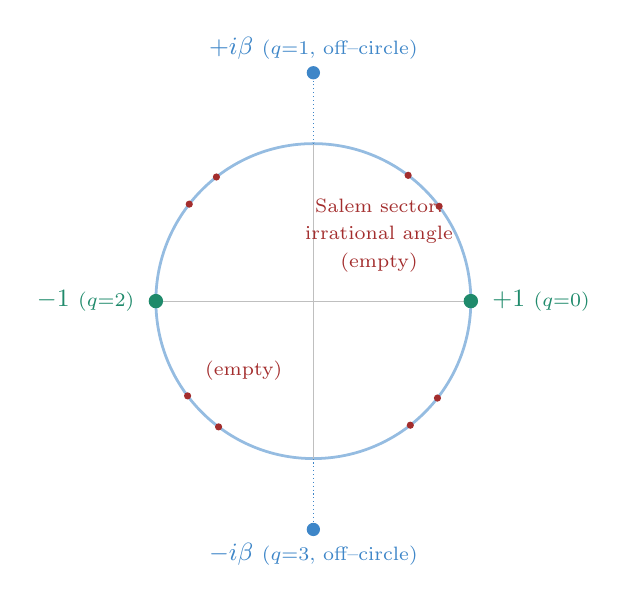
\begin{tikzpicture}[scale=1.0,>=Latex]
\draw[capc!55,line width=1pt] (0,0) circle (2);
\foreach \ang in {0,90,180,270}{ \draw[gray!50] (0,0)--(\ang:2.0); }
\fill[growc] (0:2) circle (2.6pt); \node[growc,right] at (0:2.15){\small $+1$\ \scriptsize($q{=}0$)};
\fill[growc] (180:2) circle (2.6pt); \node[growc,left] at (180:2.15){\small $-1$\ \scriptsize($q{=}2$)};
\fill[capc] (90:2.9) circle (2.4pt); \node[capc,above] at (90:2.95){\small $+i\beta$\ \scriptsize($q{=}1$, off--circle)};
\fill[capc] (270:2.9) circle (2.4pt); \node[capc,below] at (270:2.95){\small $-i\beta$\ \scriptsize($q{=}3$, off--circle)};
\draw[capc,densely dotted] (90:2)--(90:2.9); \draw[capc,densely dotted] (270:2)--(270:2.9);
\foreach \a in {37,53,128,142,217,233,308,322}{ \fill[openc] (\a:2) circle (1.3pt); }
\node[openc,align=center] at (45:1.18){\scriptsize Salem sector:\\[-2pt]\scriptsize irrational angle\\[-2pt]\scriptsize (empty)};
\node[openc] at (225:1.25){\scriptsize (empty)};
\end{tikzpicture}
\caption{\small The $\Z/4\Z$ angle charge. The four directions $\{0,\tfrac\pi2,\pi,\tfrac{3\pi}2\}$ are the roots of the content polynomial $x^4-1$. Realized on--circle: $\pm1$ (charges $0,2$, \textcolor{growc}{green}). The $\pm i$ sector (charges $1,3$) is realized only \emph{off} the circle, as $K$'s place $\pm i\beta$ (\textcolor{capc}{blue}) --- the full group is in the charge, only $\Z/2\Z$ on the circle. Every irrational angle (\textcolor{openc}{red}) is the Salem sector, off the charge lattice and empty.}
\label{fig:charge}
\end{figure}

\section{Object III: the gap (the cost floor \texorpdfstring{$\varphi$}{phi})}\label{sec:gapIII}

A conserved charge that empties a sector turns that emptiness into a quantitative bound on the realized complement. Here the bound is the cost floor.

\begin{proposition}[The base gap]\label{prop:basegap}
No monic integer quadratic $x^2+bx+c$ has Mahler measure in the open interval $(1,\varphi)$; the smallest measure exceeding $1$ is exactly $\varphi$, at $x^2-x-1$. \computed{} {\small(enumeration over $\abs b,\abs c\le6$: band $(1,\varphi)$ empty; realized values begin $\varphi,\,2,\,1{+}\sqrt2,\,\varphi^2,\,1{+}\sqrt3,\,3,\dots$)}
\end{proposition}

\begin{corollary}[The generated floor]\label{cor:floor}
Since the operators map $\{1\}\cup[\varphi,\infty)$ into itself ($\oplus$ multiplies measures, squaring squares them, $\otimes$ composes; companion paper, Lem.~6.2) and no Salem number is emitted (the off--charge sector is empty), the Mahler spectrum of $\Scal$ is $\{1\}\cup[\varphi,\infty)$, and the description--length cost carries the uniform floor $\lambda\log\varphi>0$ at every size. \forced
\end{corollary}

This is the void as a bound. The forbidden band $(1,\varphi)$ in measure space is the height image of the off--charge sector --- a sub--$\varphi$ Salem is the only thing that could populate it --- and its emptiness is the floor. The number $\varphi$ appears as the right edge of the gap: the smallest realizable growth above the trivial $\Mah=1$.

\section{Object IV: the graded normal form}\label{sec:normalIV}

The grading induces a canonical factorization of every emittable object along the charge.

\begin{proposition}[Graded normal form]\label{prop:normal}
Every object of $\Scal$ factors over $\Z$ as
\[
P\ =\ \underbrace{C(x)}_{\text{on--circle},\ C\mid x^4-1}\ \cdot\ \underbrace{G(x)}_{\text{off--circle},\ \Mah(G)=\Mah(P)\ge\varphi},
\]
with $C$ a product of $\Phi_1,\Phi_2,\Phi_4$ and $G$ splitting further by charge into a real (charges $0,2$) grow factor and, when $K$ is present, an imaginary--axis (charges $1,3$) factor. \computed
\end{proposition}

The three diagnostic cases:
\begin{center}
\renewcommand{\arraystretch}{1.25}
\begin{tabular}{@{}lll@{}}
\toprule
object & graded factorization & sectors \\
\midrule
$\varphi\otimes\varphi$ & $(x+1)^2\,(x^2-3x+1)$ & $\Phi_2^2$ (on--circle, $q{=}2$) $\times$ grow $\Mah{=}\varphi^2$\\
$\varphi^4\otimes\varphi^4$ & $(x-1)^2\,(x^2-47x+1)$ & $\Phi_1^2$ (on--circle, $q{=}0$) $\times$ grow $\Mah{=}46.98$\\
$K\otimes K$ & $(x^2+5)^4\,(x^2-5x-5)^2(x^2+5x-5)^2$ & imaginary $q{=}1,3$ $\times$ grow $\Mah{=}5.854$\\
\bottomrule
\end{tabular}
\end{center}
The first two are pure cyclotomic--times--grow; the third shows the $K$--sector $(x^2+5)$ (roots $\pm i\sqrt5$, charge $\pm\tfrac\pi2$, off circle) as the third graded piece. In all cases the on--circle part divides $x^4-1$ and the growth lives entirely in the off--circle real factor. The normal form is the structural reason the slot is empty: a Salem is \emph{irreducible} with on--circle conjugates at irrational angle, but the charge forces every emittable object into this \emph{reducible}, charge--sorted shape, in which on--circle roots are roots of unity. Irreducibility and the grading are incompatible.

\section{Object V: the conserved current}\label{sec:currentV}

Objects I--IV are static structure. Object V is the same charge read dynamically, and we are explicit about what that adds and what it does not.

\begin{proposition}[Block--diagonal evolution]\label{prop:current}
Any evolution of $\Scal$ built from the operators is block--diagonal with respect to the $\Z/4\Z$ grading: it cannot carry amplitude from one charge sector to another. Hence the charge is a constant of motion, and no admissible dynamics --- iteration of $\oplus,\otimes,(\cdot)^2$, or the monodromy of any closed parameter loop --- transitions into the off--charge sector. \forced
\end{proposition}

As a statement, Proposition~\ref{prop:current} is the conservation law of Theorem~\ref{thm:charge} restated in dynamical language; it is thinner than Objects I--IV, and we say so plainly. What it adds beyond restatement is one verified consequence.

\begin{proposition}[Clean radial growth]\label{prop:clean}
Under iteration of the operators, every Mahler measure stays in $\{1\}\cup[\varphi,\infty)$ --- never the forbidden band $(1,\varphi)$ --- and every on--circle root stays a root of unity. \computed{} {\small(two generations deep: measures $\varphi,\varphi^2,\varphi^4,46.98,76.63,122.99,8049.92,\dots$, on--circle parts roots of unity throughout)}
\end{proposition}

So the floor of Object III is not only a static fact about the spectrum but a dynamical invariant of the orbit: because the on--circle sector is frozen (roots of unity, measure $1$) and growth is confined to the off--circle grow factor, the measure evolves multiplicatively within $\{1\}\cup[\varphi,\infty)$ at every step. The growth is clean --- radial, charge--preserving, floor--respecting. The remaining dynamical content, the \emph{boundary} flow that carries a would--be occupant presented at the sector edge to a totally real Perron point with a $\sqrt5$ limit, is the trace redirection $\beta\mapsto\beta+\beta^{-1}$; that is the subject of the companion paper \emph{The Occupant of the Salem Slot} and is not reproduced here.

\section{Minimality: the floor is derived, not posited}\label{sec:minimal}

Each generated object is the smallest of its kind, because each input is forced to its minimal value --- and the output that matters most is the floor.

\begin{proposition}[The minimal chain]\label{prop:minimal}
The generating data are forced and minimal in sequence:
\begin{enumerate}[leftmargin=1.6em,itemsep=1pt]
\item \textbf{Degree two} is the unique degree whose self--action realizes a ternary decision: $\#\text{channels}(d)=d^2-d+1=3$ iff $d=2$, with the centralizer the inseparable $0$--channel. (Companion paper, ternary lock.)
\item \textbf{Order four} is the charge: $\tfrac\pi2\Z\cong\Z/4\Z$ is the coarsest quantization carrying a ``fourth direction'' distinct from the three real channels, and its $\pm i$ generator enters through the quartic field $\Q(5^{1/4})$ --- whose splitting field contains $i$ --- i.e.\ through the same $K$ that is the construction's one Lorentzian seed.
\item \textbf{The floor $\varphi$} is the output: the smallest Perron number, the smallest Mahler measure of a non--cyclotomic integer quadratic, the right edge of the minimal gap.
\end{enumerate}
\forced
\end{proposition}

Read in the forced direction, the chain says something specific about the floor, and it is worth stating without ornament. The framework posits one thing about growth decisions --- that they are ternary --- and ternary arity forces degree two (Proposition~\ref{prop:minimal}(1)). The cost floor $\varphi$ is then \emph{not an input}: it is the smallest realizable growth above the trivial, forced out the far end of the construction (Proposition~\ref{prop:basegap}). $\varphi$ was not chosen for being golden; degree--two decisions were chosen, and $\varphi$ is what they produce. The floor is a consequence of the decision arity, not an assumption adjoined to it.

That is the whole content of the minimality result: in this construction the golden ratio is \emph{derived}. The chain $\text{degree }2\Rightarrow\Z/4\Z\Rightarrow\varphi$ is three forced minima producing three forced outputs --- the smallest grading, the smallest content polynomial $x^4-1$, the smallest gap --- and the appearance of $\varphi$ at the end is the theorem, not a hypothesis. This is the load--bearing result of the paper, and its weight is exactly that and no more: a floor that the decision structure forces, in one fully computable instance.

\section{Scope: a universal pattern, a local instance}\label{sec:scope}

The equivalence of \S\ref{sec:substrate} is domain--universal; the five objects of \S\S\ref{sec:gradingI}--\ref{sec:currentV} are local. Both halves matter, and conflating them is the error to avoid.

\begin{center}
\renewcommand{\arraystretch}{1.25}
\begin{tabular}{@{}p{0.20\linewidth} p{0.26\linewidth} p{0.20\linewidth} p{0.22\linewidth}@{}}
\toprule
domain & conserved charge & empty sector & what the emptiness generates \\
\midrule
fermions (QM) & wavefunction antisymmetry & doubly--occupied states & shell structure, degeneracy pressure \\
charge superselection (QFT) & total charge & cross--sector coherences & block structure of observables \\
type theory & subject reduction & ill--typed states & ``illegal states unrepresentable,'' optimizations \\
emission algebra (here) & angle charge $\Z/4\Z$ & the Salem slot & $x^4-1$, the floor $\varphi$, the graded normal form \\
\bottomrule
\end{tabular}
\end{center}

The table is to be read \emph{down each column}, never causally across rows. What is shared is the \emph{skeleton}: a conserved charge makes a sector kinematically empty, and the emptiness organizes the realized complement (a grading, a content alphabet, a gap, a normal form, a conserved current). Each row's output is that row's own --- the shell structure is a fact about antisymmetric fermions, $x^4-1$ is a fact about the angle charge --- and no row's output is derived from, or explains, another's. In particular nothing here is a claim that the angle charge $\Z/4\Z$ explains Pauli exclusion, or that the periodic table and $x^4-1$ share more than the structural form of ``forbidden sector organizes the realized complement.'' Pauli exclusion is the most familiar instance of the \emph{skeleton} --- an antisymmetry charge whose forbidden sector has zero amplitude, never violated --- and it is invoked only at that structural level.

What does not transfer is the content. The five objects this charge generates --- $x^4-1$, the floor $\varphi$, the graded factorization, the trace flow with its $\sqrt5$ limit --- are theorems of \emph{this} number theory, not exported engines for other fields. The only genuinely portable mathematics beyond the pattern is the \emph{local} differential structure: a two--to--one cover with a fold has a square--root branch point generically (Chebyshev maps, modular curves, mapping--class monodromy), so the $\sqrt{t-2}$ edge and the $\beta\leftrightarrow\beta^{-1}$ monodromy recur widely; but $\sqrt5=\varphi+\varphi^{-1}$, the identification of the floor's image with the grow generator, is this construction's own. The honest statement is precise: the substrate (kinematic emptiness $\equiv$ conserved charge $\equiv$ superselection) is one of the most generative patterns there is, and the Salem slot is a clean, minimal, fully computable realization of it --- a generator of its own domain's structure, exhibiting in the small what the pattern does at large.

\section{Epistemic ledger}\label{sec:ledger}

\begin{center}
\renewcommand{\arraystretch}{1.18}
\begin{tabular}{@{}p{8.2cm}cl@{}}
\toprule
\textbf{Claim} & \textbf{Status} & \textbf{Backing}\\
\midrule
Kinematic vs.\ dynamic emptiness; the substrate equivalence & \declared & Def.~\ref{def:two}, \S\ref{sec:substrate}\\
Object I --- angle charge is $\Z/4\Z$, conserved, fully realized (via $K$) & \computed & Thm.~\ref{thm:charge}\\
Operators act as add ($\otimes$), double (squaring), union ($\oplus$) & \computed & Thm.~\ref{thm:charge}\\
Object II --- content polynomial $x^4-1=\Phi_1\Phi_2\Phi_4$ & \computed & Prop.~\ref{prop:content}\\
Full $\Z/4\Z$ in the charge; only $\Z/2\Z{=}\{\pm1\}$ on the circle & \computed & Rem.~\ref{rem:algebra-not-circle}\\
Object III --- no integer quadratic with $\Mah\in(1,\varphi)$; floor $\varphi$ & \computed & Prop.~\ref{prop:basegap}, Cor.~\ref{cor:floor}\\
Object IV --- graded normal form, on--circle $\mid x^4-1$ $\times$ grow $\Mah{\ge}\varphi$ & \computed & Prop.~\ref{prop:normal}\\
Object V --- block--diagonal evolution (conservation restated) & \forced & Prop.~\ref{prop:current}\\
Object V --- clean radial growth: orbit measures in $\{1\}\cup[\varphi,\infty)$ & \computed & Prop.~\ref{prop:clean}\\
Minimal chain degree $2\Rightarrow\Z/4\Z\Rightarrow\varphi$; floor derived not posited & \forced & Prop.~\ref{prop:minimal}\\
Pattern universal (Pauli, superselection, types); content local & \declared & \S\ref{sec:scope}\\
$\sqrt5=\varphi+\varphi^{-1}$ local; $\sqrt{\cdot}$ branch \& monodromy portable & \forced & \S\ref{sec:scope}\\
\bottomrule
\end{tabular}
\end{center}

\paragraph{Summary.} A kinematic void --- a sector emptied by a conserved charge rather than guarded by a barrier --- is a generator. On the minimal instance, the angle charge $\Z/4\Z$ of the Salem slot produces five canonical objects: the grading (I), the content polynomial $x^4-1$ (II), the cost floor $\varphi$ (III), the graded cyclotomic--times--grow normal form (IV), and the conserved current whose dynamical content is clean radial growth (V). The floor is the result that carries weight: degree two is forced by ternary arity, and $\varphi$ falls out the far end as the minimum realizable growth, so the golden ratio is derived from the decision structure rather than posited. The pattern beneath --- kinematic emptiness $\equiv$ conserved charge $\equiv$ superselection --- is the same skeleton that, in each domain, does that domain's own work: for fermions the shell structure, for type systems their correctness, here the five objects; the skeleton is shared, the outputs are not exported. The void does not merely sit there refusing to be filled. Refusing to be filled, in a conserved way, is the act of generation.

\end{document}
